\chapter{Termo de Abertura do projeto}

\section{EAP}
\begin{figure}[!htb]
    \center{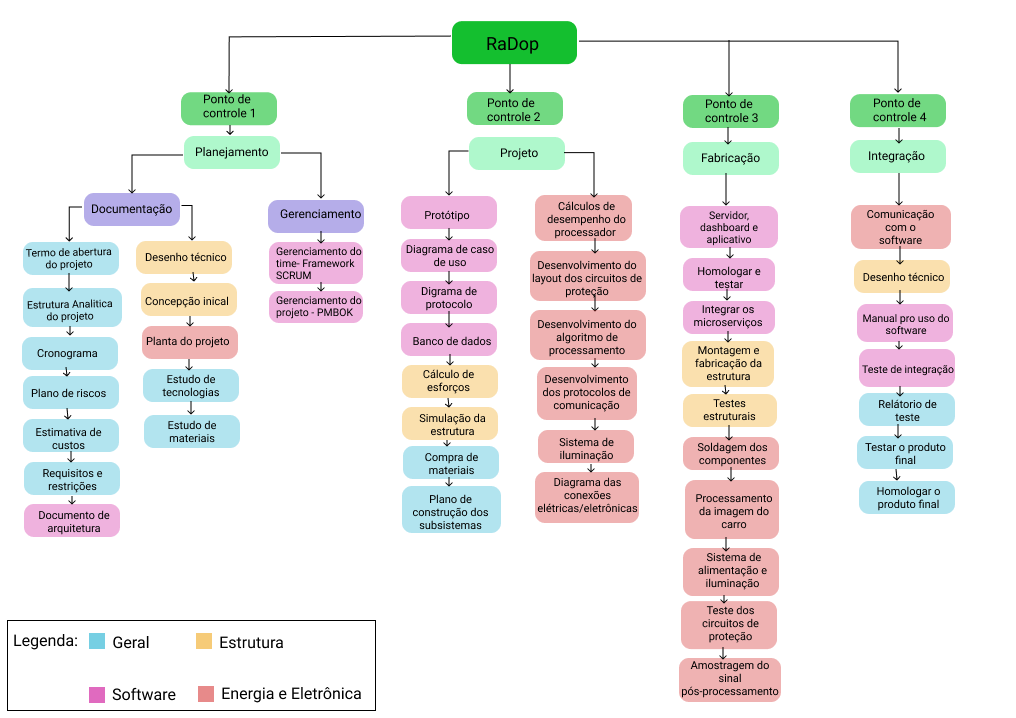
\includegraphics[width=\textwidth]{eap.eps}}
    \caption{\label{fig:eap} EAP do projeto}
\end{figure}
\section{Lista É/Não é}
\subsection{É}
\subsection{Não é}
\section{Requisitos}
\subsection{Eletrônica}
\subsection{Energia}
\begin{itemize}
	\item O sistema deve conter painéis fotovoltaicos que promoverão a fonte de alimentação para todos os componentes do sistema;
	\item O sistema deve garantir o máximo aproveitamento energético;
	\item O sistema deve conter circuitos de controle de tensão e corrente;
	\item O sistema deve conter circuitos de controle de tensão e corrente;
	\item O sistema deve garantir o funcionamento seguro e contínuo do Radar;
	\item O sistema deve conter um circuito de iluminação para servir de alerta aos motoristas;
	\end{itemize}

	\vspace*{\fill}
    \pagebreak
    
\subsection{Estrutura}
\subsection{Software}
\section{\emph{Stakeholders}}
\section{Recurso humanos}
\section{Cronograma de atividades}



\section{Milestones Identificados}
\section{Estimativa de custos}
\section{Viabilidades financeira}
\section{Levantamento de riscos}
<<<<<<< HEAD
=======

\begin{comment}
\begin{description}
	\item [Pré-textuais] \

	\begin{itemize}
		\item Capa
		\item Folha de rosto
		\item \textit{Dedicatória}
		\item \textit{Agradecimentos}
		\item \textit{Epígrafe}
		\item Resumo
		\item Abstract
		\item Lista de figuras
		\item Lista de tabelas
		\item Lista de símbolos e
		\item Sumário
	\end{itemize}

	\item [Textuais] \

	\begin{itemize}
		\item \textbf{\textit{Introdução}}
		\item \textbf{\textit{Desenvolvimento}}
		\item \textbf{\textit{Conclusões}}
	\end{itemize}

	\item [Pós-Textuais] \
	
	\begin{itemize}
		\item Referências bibliográficas
		\item \textit{Bibliografia}
		\item Anexos
		\item Contracapa
	\end{itemize}
\end{description}

\end{comment}

>>>>>>> 4ef4c5a9d179b0ced8d6ff52122a2aacd641c19d
